\section{Experimental Evaluation and Limitations}
\label{sec:evaluation}

\lstset{basicstyle=\ttfamily}

In this section, we first test our approach on the running example presented in Section~\ref{sec:running_example}. We then run a user-based evaluation to validate our approach. Next, we evaluate a real-world BOLA-vulnerable open source software with our tool. Finally, we describe the threats to validity of our approach. 

\subsection{Running Example Evaluation}
\label{sec:running_example_evaluation}

Similar to other works in the literature~\cite{collado2020using,schoenborn2021detecting}, we use the OWASP Juice Shop web application to test the accuracy of vulnerability and attack detection solutions. This approach has the advantages of providing a controlled environment without data noise, while ensuring similar characteristics to a real-world environment. %In this section we will present the test environment used, the test cases and results obtained.

The first step is to instrument OWASP Juice Shop to generate event logs. This code can be found publicly available at GitHub\footnote{Accessible in \url{https://github.com/ailton07/juice-shop-with-winston}.}. We then deployed the application to an AWS EC2 instance, a cloud service that allows the creation of a virtual server to run applications on the Amazon Web Services infrastructure, making the application accessible via URL of type \url{http://ec2-XXX-XXX-XXX-XXX.compute-1.amazonaws.com:3000}, where the \textit{X} represent the public IP of the running instance. 

Now, we reproduce the attacks on the Juice Shop vulnerabilities related to BOLA. The Juice Shop was created with the following vulnerabilities related to BOLA:
\begin{enumerate}[{\sc {Vulnerability} 1.}]
    \item \textit{View cart}, which consists of viewing another user's shopping cart; %(View another user's shopping cart)
    \item \textit{Manipulate cart}, which consists of placing a product in another user's shopping cart.
\end{enumerate}



The guide to successfully exploring such vulnerabilities is publicly available\footnote{See \url{https://pwning.owasp-juice.shop/appendix/solutions.html}.}. Following these steps, the scenario for the first challenge is that upon loading the website and logging in, a \textit{POST} request is sent to the \textit{/rest/user/login} API endpoint, returning the user's token to the client and user cart identifier (called \textit{bid}). After this, the home page of the website is displayed. One of the requests sent in this process is \textit{GET /rest/basket/6}, where the value $6$ refers to the shopping cart identifier obtained in the login request. The attack consists of sending \textit{GET} requests to \textit{/rest/basket/} with a different shopping cart identifier than the one received in the login process  after loading the home page. According to the guide, adding or subtracting $1$ from its value is enough to explore the vulnerability.

The log file obtained after performing the account registration, login, and exploit attack process is publicly available on our GitHub~\cite{links2cpn}. This 30-line log file is processed and transformed using the algorithms described in Section~\ref{sec:transformation}. The obtained CPN is then verified with the replay algorithm as explained in Section~\ref{sec:detecting_bola}. 

As a result, we got the nets shown in Figure~\ref{fig:Juice_Shop_output_challenge1}  and the error message shown in Listing~\ref{lst:challenge1_error_msg}. Figure~\ref{fig:Juice_Shop_output_challenge1_a} shows the initial state of the CPN, being the immediate result of the transformation from OpenAPI to CPN. Likewise, 
Figure~\ref{fig:Juice_Shop_output_challenge1_b} shows the status of the CPN after processing the line of the log file that represents the request \textit{POST /rest/user/login} with response $ bid=6$. Finally, 
Figure~\ref{fig:Juice_Shop_output_challenge1_c} shows the CPN status after processing the line that represents the \textit{GET /rest/basket/6} request. Listing~\ref{lst:challenge1_error_msg} ilustrate the processing of the line that represents the request \textit{GET /rest/basket/7} , which is the BOLA attack we performed. This error message briefly states that there is no token available at the CPN's place to make the transition enabled.

\begin{figure*}
     \centering
    \begin{subfigure}[b]{0.3\textwidth}
        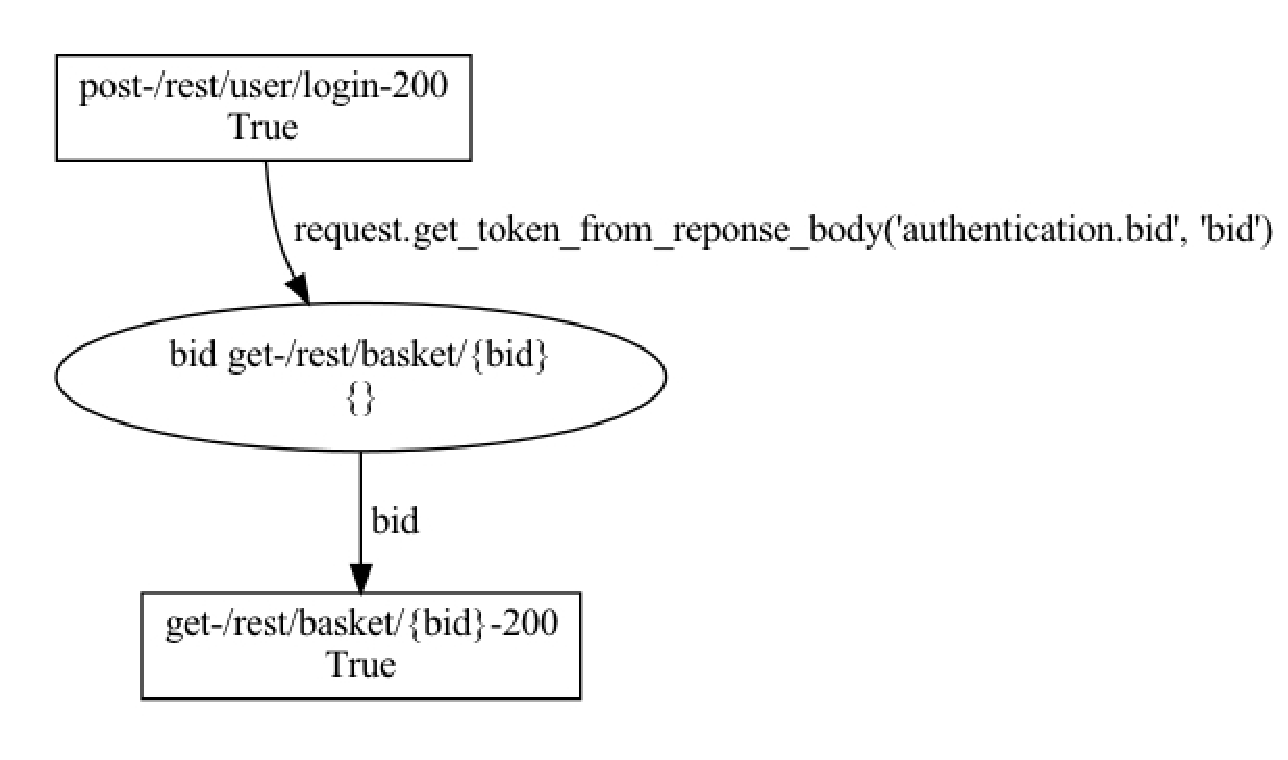
\includegraphics[width=\textwidth]{figures/Juice_Shop_output_challenge1_a}
        \caption{Initial state of the CPN}
        \label{fig:Juice_Shop_output_challenge1_a}
    \end{subfigure}
        \begin{subfigure}[b]{0.3\textwidth}
        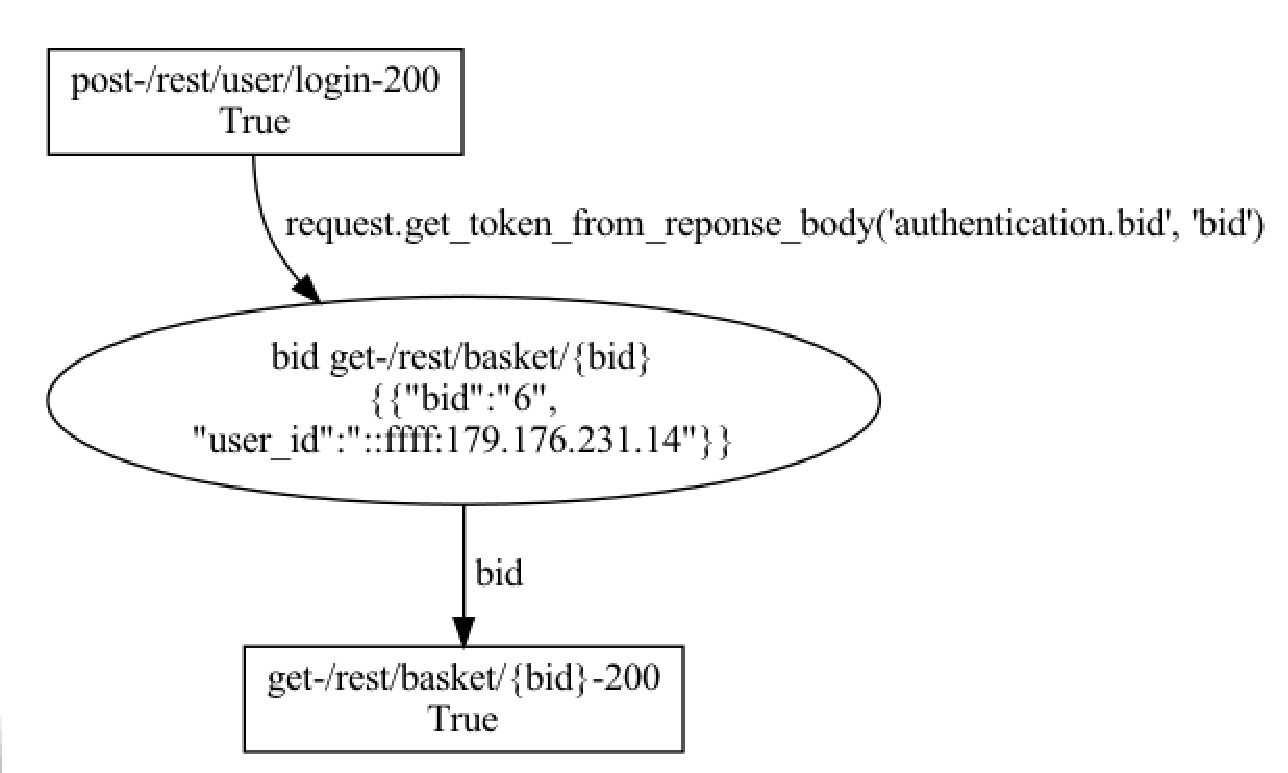
\includegraphics[width=\textwidth]{figures/Juice_Shop_output_challenge1_b}
        \caption{State of the CPN after processing \textit{POST /rest/user/login} (with response $bid=6$)}
        \label{fig:Juice_Shop_output_challenge1_b}
    \end{subfigure}
        \begin{subfigure}[b]{0.3\textwidth}
        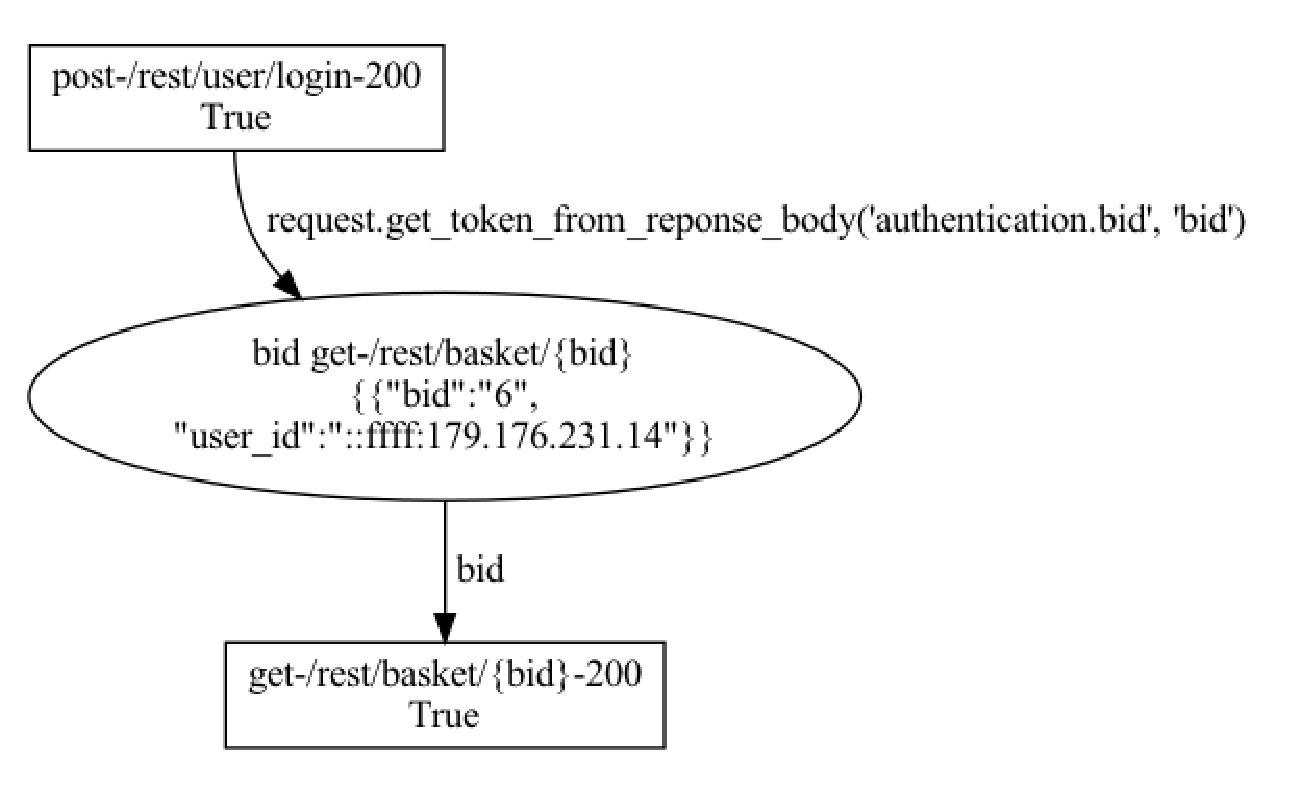
\includegraphics[width=\textwidth]{figures/Juice_Shop_output_challenge1_c}
        \caption{State of the CPN after processing \textit{GET /rest/basket/7}}
        \label{fig:Juice_Shop_output_challenge1_c}
    \end{subfigure}
    \caption{Result of running the transformation algorithms on the event log for {\sc Vulnerability 1}.}
    \label{fig:Juice_Shop_output_challenge1}
\end{figure*}

\begin{lstlisting}[caption={Error message received when executing challenge 1},captionpos=t,basicstyle=\ttfamily\small, label={lst:challenge1_error_msg},frame=single,breaklines=true]
Fire error, line 29:  transition not enabled for 
{
   "bid ->"{
      "bid":"None",
      "user_id":"::ffff:179.176.231.14"
   },
   "request ->"{
      "uri":"/rest/basket/7",
      "method":"GET",
      "user_id": "::ffff:1..."}
}
\end{lstlisting}


Following the same guide to successfully attacking {\sc Vulnerability 2}, after the website loads and the user logs in, a \textit{POST} request is sent to the \textit{/rest/user/login} API endpoint, returning the user's token to the client's and user's cart identifier (called \textit{bid}), similar to {\sc Vulnerability 1}. After this, the home page of the website is displayed. By clicking on any product and adding it to the shopping basket via the \textit{Add to Basket} button, a \textit{POST} request is sent to the  \textit{/api/BasketItems/} API endpoint with the values \textit{ProductId} (product code), \textit{BasketId} (identifier of the user's basket) and \textit{quantity} (quantity of the product to add). The attack consists of sending \textit{POST} requests to \textit{/api/BasketItems/} with a different shopping cart identifier than the one received at login, in addition to the one already present. According to the guide, adding or subtracting $1$ from its value is enough to exploit the vulnerability.

The log file obtained after performing the account registration, login, and exploit attack process is publicly available on our GitHub~\cite{links2cpn}. Similarly to {\sc Vulnerability 1}, this 23-line log file is processed and transformed using the algorithms described above, and the obtained CPN is verified with the replay algorithm, as explained in Section~\ref{sec:detecting_bola}. 

\begin{lstlisting}[caption={Error message received when executing challenge 2}, captionpos=t,basicstyle=\ttfamily\small, label={lst:challenge2_error_msg},frame=single,breaklines=true]
Fire error, Line 21: POST /api/BasketItems/ 200 11ms
transition not enabled for
{
   "BasketId ->"{
      "BasketId":"5",
      "user_id":"::ffff:35.199.121.33"
   },
   "request ->"{
      "uri":"/api/BasketItems/",
      "method":"POST",
      "user_id":"::ff...
   }
}
\end{lstlisting}


As a result, we got the nets shown in Figure~\ref{fig:Juice_Shop_output_challenge2}  and the error message shown in Listing~\ref{lst:challenge2_error_msg}. Figure~\ref{fig:Juice_Shop_output_challenge2_a} shows the initial state of the CPN, being the immediate result of the transformation from OpenAPI to CPN. In addition, Figure~\ref{fig:Juice_Shop_output_challenge2_b} shows the CPN status after processing the log file line that represents the \textit{POST /rest/user/login} request with response $bid=6$. Listing~\ref{lst:challenge2_error_msg} illustrates the processing of the line $21$, which represents the \textit{POST /api/BasketItems/} request regarding the BOLA attack we performed. This error message briefly indicates that there is no token available at the CPN place to enable the firing of the transition.


\begin{figure*}
    \centering
    \begin{subfigure}[b]{0.49\textwidth}
        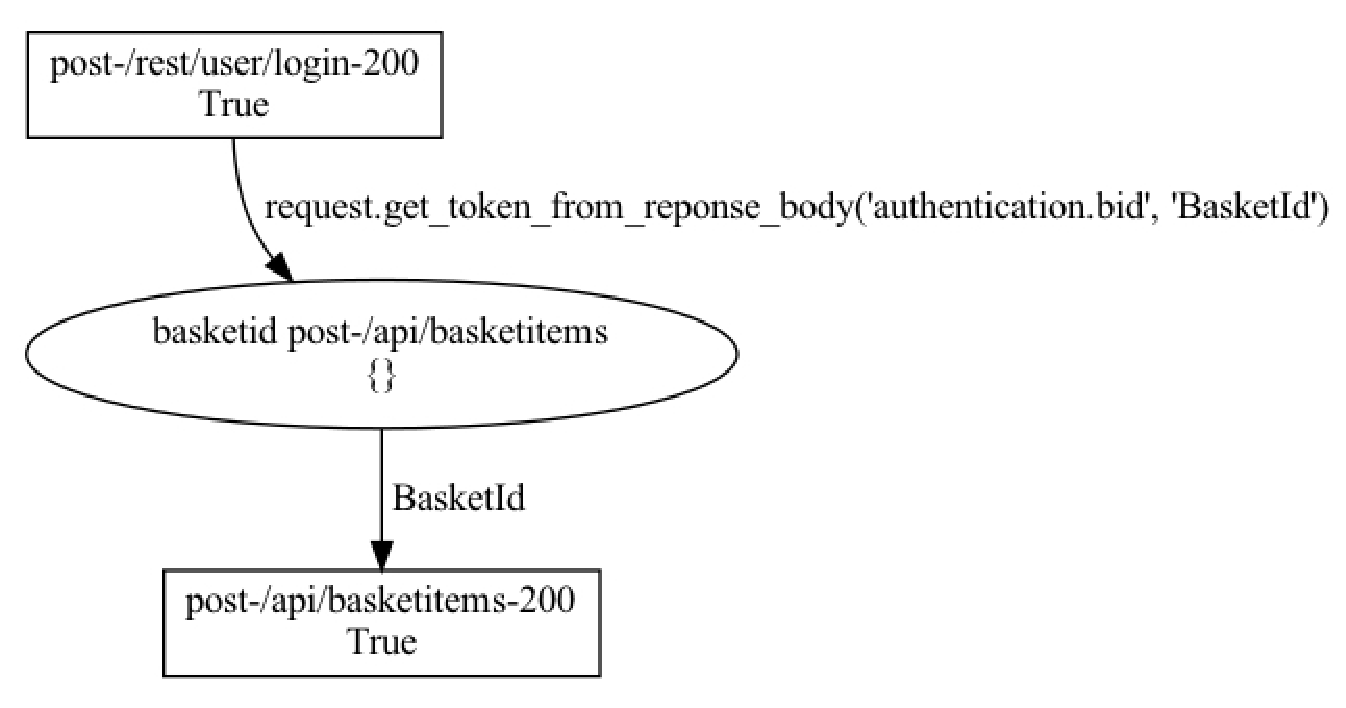
\includegraphics[width=\textwidth]{figures/Juice_Shop_output_challenge2_a}
        \caption{Initial state of the CPN}
        \label{fig:Juice_Shop_output_challenge2_a}
    \end{subfigure}
    \begin{subfigure}[b]{0.49\textwidth}
        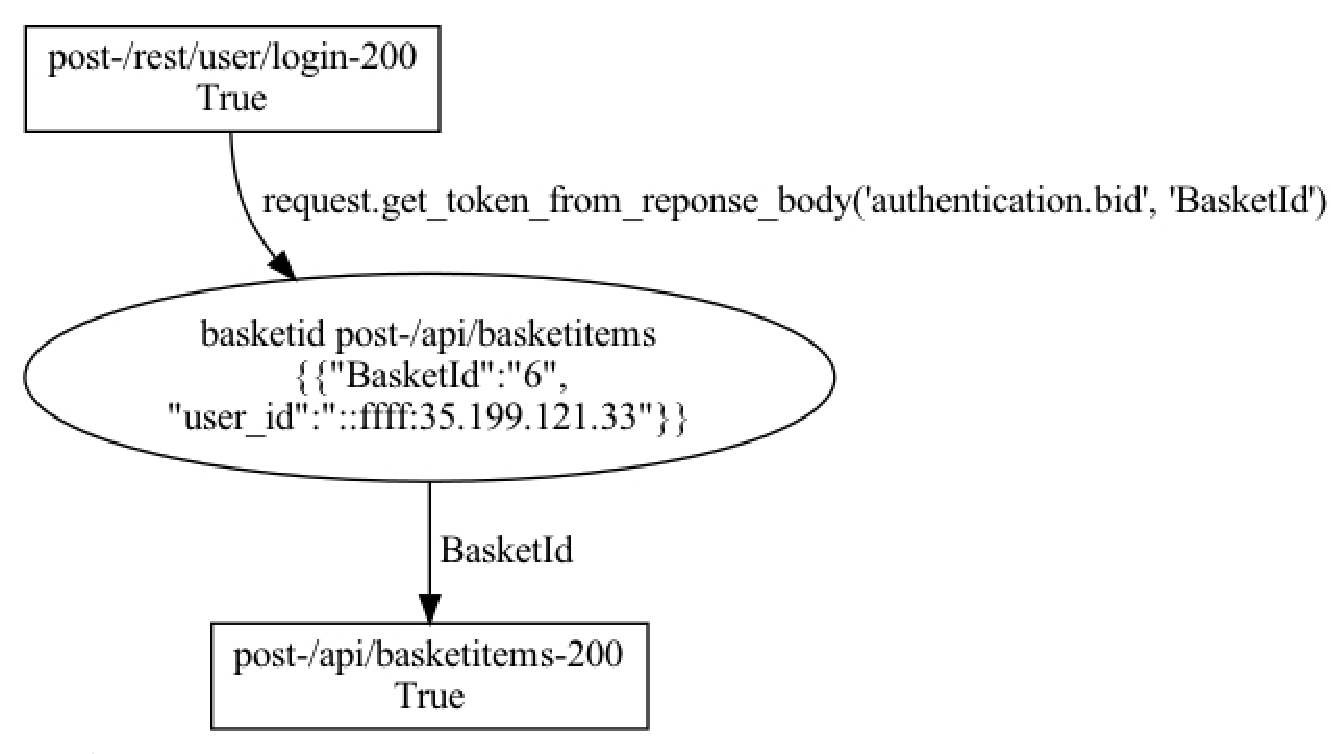
\includegraphics[width=\textwidth]{figures/Juice_Shop_output_challenge2_b}
        \caption{State of the CPN after processing \textit{POST /rest/user/login} (with response $bid=6$)}
        \label{fig:Juice_Shop_output_challenge2_b}
    \end{subfigure}
    \caption{Result of running the transformation algorithms on the event log for {\sc Vulnerability 2}.}
    \label{fig:Juice_Shop_output_challenge2}
\end{figure*}


\subsection{User-Based Evaluation}
\label{sec:ruser_based_evaluation}

To test the proposed solution in a more realistic scenario, we have carried out a user-based evaluation. 
%To do this, we invited 15 Computer Science students from the Computer Network Security course to try to exploit 
For this, we invited Computer Science students from the Federal University of Amazonas, enrolled in the Computer Network Security discipline (ICC303), to try to exploit
{\sc Vulnerability 1} and {\sc Vulnerability 2} described in Section~\ref{sec:running_example_evaluation}.
There were $20$ students enrolled in the discipline and $15$ attending to the end, who were the ones invited for this evaluation.

As a test environment, we set up an instance of the Juice Shop application (see Section~\ref{sec:running_example})  running on an AWS Web server (EC2) from January 25, 2023 to February 8, 2023. We first explain the basics of the BOLA vulnerability and give examples of exploitation. We then explain the Juice Shop app and instruct students to exploit both vulnerabilities in the shopping cart as they see fit, writing reports on the process. We also advise them not to copy solutions from the Internet, but to try to build their own exploits of the vulnerabilities.

In the end, we got 12 attack reports, approximately $4,000$ log lines, $2,000$ requests analyzed, 514 requests associated with {\sc Vulnerability 1} %(\textit{GET /rest/basket/}) 
and 192 requests associated with {\sc Vulnerability 2}% (\textit{ POST/api/BasketItems/})
. For each of the reports received, we manually analyze the generated logs, especially those associated with registration process, the login process, {\sc Vulnerability 1}, and {\sc Vulnerability 2}. Thanks to this manual analysis, we are able to calculate the number of legitimate requests, the number of of attack attempts and the number of successful attacks.  
%
Subsequently, we process the generated logs with our tool (introduced in Section~\ref{sec:methodology}) to obtain the requests classified as legitimate and as attacks, and compare them with the data obtained through our manual analysis. 

As a result, we get the data shown in Table~\ref{table:attacks_summary}. For \textsc{Vulnerability 1} ({\sc V1}), \textit{Total Requests} refers to the number of requests logged in \texttt{GET /rest/basket/}, while for \textsc{Vulnerability 2} ({\sc V2}), it refers to the number of requests logged in \texttt{POST /api/BasketItems/}. Recall the description of both vulnerabilities in Section~\ref{sec:running_example_evaluation}. \textit{Attack Attempts} refers to the number of requests that we manually classified as attacks (failed and successfully) on the cited endpoints, while \textit{Successful Attacks} refers to the number of requests that were manually classified as successful attacks. Finally, \textit{Requests classified as attacks} refers to the number of requests that were classified by our tool as attacks on the cited endpoints.

After that, we processed the logs generated with the proposed solution in order to obtain the list of requests classified as legitimate and as attacks, and compare them with the data obtained through manual analysis.
We then obtained the data shown below in Table~\ref{table:attacks_summary}. To \textit{Vulnerability 1}, \textit{Total requests} refers to the number of requests registered to \textit{GET /rest/basket/}, while \textit{Vulnerability 2} refers to the number of requests registered to \textit{POST /api/BasketItems/}. \textit{Attack attempts} refers to the number of requests that were manually classified as attacks on the cited endpoints. \textit{Successful attacks} refers to the number of requests that were manually classified as successful attacks on the cited endpoints. Finally, \textit{Requests classified as attacks} refers to the number of requests that were classified by the proposed solution as attacks on the endpoints cited.

\begin{table}
\caption{Summary of data obtained from the attacks.}
\label{table:attacks_summary}
\centering
\begin{tabular}{p{.28\columnwidth} | r r}
\cline{2-3}
 & \multicolumn{1}{c}{\cellcolor{LightGray}\textsc{V1}} &  \multicolumn{1}{c}{\cellcolor{LightGray}\textsc{V2}} \\
\hline
\cellcolor{LightGray}\textbf{Total requests}                 & 517                      & 192                      \\ 
\cellcolor{LightGray}\textbf{Attack attempts}                & 101                      & 100                      \\ 
\cellcolor{LightGray}\textbf{Successful attacks}             & 98                       & 20                       \\ 
\cellcolor{LightGray}\textbf{Requests classified as attacks} & 101                      & 25                       \\
\hline
\end{tabular}
\end{table}

To express the performance of our approach, we calculate the standard metrics of $\text{\em Accuracy}=\frac{TP + TN}{TP + FP + FN + TN}$, $\text{\em Precision}=\frac{TP}{TP + FP}$, $\text{\em Recall}=\frac{TP}{TP + FN}$, $\text{\em F1-score}=\frac{2\cdot\text{\em Recall}\cdot\text{\em Precision}}{\text{\em Recall} + \text{\em Precision}}$. In this setting, false positives ($FP$) refer to benign requests that are wrongly classified as attacks, false negatives ($FN$) refer to attack requests that have not been classified as attacks, true positives ($TP$) refer to benign requests that are correctly classified as benign requests, and true negatives ($TN$) refer to attack requests that are correctly classified as attack requests.


%\begin{equation}
%\begin{split}
%\text{\em Accuracy}&=\dfrac{TP + TN}{TP + FP + FN + TN}\\
%\text{\em Precision}&=\dfrac{TP}{TP + FP}\\
%\text{\em Recall}&=\dfrac{TP}{TP + FN}\\
%\text{\em F1-score}&=\dfrac{2\cdot\text{\em Recall}\cdot\text{\em Precision}}{\text{\em Recall} + \text{\em Precision}}\\
%\end{split}
%\end{equation}

%\noindent where $TP$ is the number of true positives, $TN$ is the number of true negatives,  $FP$ is the number of false positives, and $FN$ is the number of false negatives.

The confusion matrix is show in Table~\ref{table:confusion_matrices}(a). For {\sc V1}, we obtain \(\text{\em Accuracy} = \text{\em Precision} = \text{\em Recall} = \text{\em F1-score} = 1\), while for {\sc V2}, we obtain \(\text{\em Accuracy}= 0.609375; \text{\em Precision} = 1; \text{\em Recall = 0.25}; \text{\em F1-score} = 0.4\). In both cases, {\em Precision} remains constant, indicating consistency in classifying correctly positive cases. On the contrary, {\em Accuracy}, {\em Recall}, and {\em F1-score} vary considerably.


To investigate the divergence in performance metrics between {\sc V1} and {\sc V2}, we create the confusion matrix comparing successful attacks and those classified by our approach. The results are summarized in Table~\ref{table:confusion_matrices}(b). In this case, we obtain \(\text{\em Accuracy} = 0.9942;\) \(\text{\em Precision} = 0.97;\) \(\text{\em Recall} = 1;\) 
\(\text{\em F1-score} = 0.985\) for \textsc{Vulnerability 1}, while for \textsc{Vulnerability 2} we obtain \(\text{\em Accuracy} = 0.974;\) \(\text{\em Precision}  = 0.8; \text{\em Recall} = 1; \text{\em F1-score}  = 0.888\). These results indicate that our approach works better in detecting successfully executed attacks, rather than detecting attempted (failed and successful) attacks.

\begin{table*}
\caption{Confusion matrices.}
\label{table:confusion_matrices}
\centering
\begin{tabular}{c c}

\begin{tabular}{c cc|cc|}
\cline{4-5}
& &                   & \multicolumn{2}{|c|}{\cellcolor{LightGray}\textbf{Predicted}}                                  \\
\cline{4-5} 
& &                   & \cellcolor{LightGray}\textbf{Positive} & \cellcolor{LightGray}{\textbf{Negative}}\\
\hline
 \cellcolor{LightGray}& \cellcolor{LightGray} & \cellcolor{LightGray}\textbf{Positive} & 101             & 0                                      \\ 
 \cellcolor{LightGray} & \parbox[t]{2mm}{\multirow{-2}{*}{\rotatebox[origin=c]{90}{\cellcolor{LightGray}\sc V1}}} & \cellcolor{LightGray}\textbf{Negative} & 0                 & 416                                    \\
\cline{2-5}
\cellcolor{LightGray}& \cellcolor{LightGray} & \cellcolor{LightGray}\textbf{Positive} & 25             & 75 \\ 
\parbox[t]{2mm}{\multirow{-4}{*}{\rotatebox[origin=c]{90}{\cellcolor{LightGray}\bf Actual}}} &
\parbox[t]{2mm}{\multirow{-2}{*}{\rotatebox[origin=c]{90}{\cellcolor{LightGray}\sc V2}}}
 & \cellcolor{LightGray}\textbf{Negative} & 0                 & 92                                    \\
\hline
\end{tabular}

& 

\begin{tabular}{c cc|cc|}
\cline{4-5}
& &                   & \multicolumn{2}{|c|}{\cellcolor{LightGray}\textbf{Predicted}}                                  \\
\cline{4-5} 
& &                   & \cellcolor{LightGray}\textbf{Positive} & \cellcolor{LightGray}{\textbf{Negative}}\\
\hline
 \cellcolor{LightGray}& \cellcolor{LightGray} & \cellcolor{LightGray}\textbf{Positive} & 98             & 0                                      \\ 
 \cellcolor{LightGray} & \parbox[t]{2mm}{\multirow{-2}{*}{\rotatebox[origin=c]{90}{\cellcolor{LightGray}\sc V1}}} & \cellcolor{LightGray}\textbf{Negative} & 3                 & 416                                    \\
\cline{2-5}
\cellcolor{LightGray}& \cellcolor{LightGray} & \cellcolor{LightGray}\textbf{Positive} & 20             & 0 \\ 
\parbox[t]{2mm}{\multirow{-4}{*}{\rotatebox[origin=c]{90}{\cellcolor{LightGray}\bf Actual}}} &
\parbox[t]{2mm}{\multirow{-2}{*}{\rotatebox[origin=c]{90}{\cellcolor{LightGray}\sc V2}}}
 & \cellcolor{LightGray}\textbf{Negative} & 5                 & 167                                    \\
\hline
\end{tabular}\\
(a) Attack attempts versus detections & (b) Successful attacks versus detections\\

\end{tabular}
\end{table*}

Our results also show that {\sc Vulnerability 1} and {\sc Vulnerability 2} actually have very different {\em attack attempt/attack success} rates. For  {\sc Vulnerability 1}, there were 98 successful attacks out of 101 attack attempts (i.e., $97.02\%$ success rate), while for {\sc Vulnerability 2}, there were 20 successful attacks out of 100 attack attempts (i.e., $20\%$ success rate). One explanation for this difference in the success rate of exploiting vulnerabilities is the difference in the difficulty of exploiting the vulnerability. According to the exploit guide of Juice Shop\footnote{Publicly available at \url{https://pwning.owasp-juice.shop/appendix/solutions.html}.}, {\sc Vulnerability 1} has 2 stars of difficulty, while {\sc Vulnerability 2} has 3 stars. This may be why 3 out of 12 students who submitted reports were unable to successfully exploit {\sc Vulnerability 2}.


\subsection{Real-World Software Evaluation}

To test the solution proposed in this work with a real application vulnerable to BOLA, we consider the {\tt Memos} application, presented previously (see Section~\ref{sec:transformation}).
As before, the first step is to instrument the {\tt Memos} API to generate event logs. The {\tt Memos} code, containing the modifications described below, is publicly available on GitHub\footnote{Accessible in \url{https://github.com/ailton07/memos-with-BOLA}}. As we have taken the latest version of {\tt Memos} as the code base, where the BOLA vulnerability is already fixed, we had to revert this fix to make the code vulnerable again.


A guide to exploiting the vulnerability is described in~\cite{huntr2022}. Following these steps,twhen the website loads and the user logs in, a {\em GET} request is sent to the {\em /api/v1/memo} endpoint, returning the notes that belong to the logged-in user. After this, the user can create a note via a {\em POST} request to the {\em /api/v1/memo} endpoint, or archive one of the notes from their notes list via a {\em PATCH} request to {\em /api/v1/memo/\{memoId\}}, where {\em \{memoId\}} is the list of note identifiers that the user wants to archive. The attack consists of sending {\em PATCH} requests to {\em /api/v1/memo/\{memoId\}} with values of {\em memoId} that does not belong to the logged-in user.


The log file obtained after performing the account registration, subsequent login, and exploit attack process is also publicly available in the software repository of our tool~\cite{links2cpn}. This 11-line log file is processed and transformed using the algorithms described in Section~\ref{sec:transformation} and the obtained CPN is verified with the replay algorithm as explained in Section~\ref{sec:detecting_bola}.

Figures~\ref{fig:Memos_attack_case_a} and ~\ref{fig:Memos_attack_case_b} shows the CPN obtained after the replay algorithm, while Listing~\ref{lst:memos_error_msg} shows the error message obtained. In particular, Figure~\ref{fig:Memos_attack_case_a} shows the initial state of the CPN, being the immediate result of the transformation from OpenAPI to CPN, while Figure~\ref{fig:Memos_attack_case_b} shows the state of CPN after processing the log file line representing the request \textit{GET /api/v1/memo} with response $memoId=3$ and $memoId=1$, and the CPN state after processing the log line representing a legitimate request. Likewise, Listing~\ref{lst:memos_error_msg} illustrates the processing of line $11$ of the log, which represents the \textit{PATCH /api/v1/memo/6} request and corresponds to the BOLA attack we performed. This error message briefly indicates that there is no token available at the CPN site to allow the transition to be fired, thus successfully detecting the occurrence of the attack.


\begin{figure*}
    \center
    \begin{subfigure}{\textwidth}
    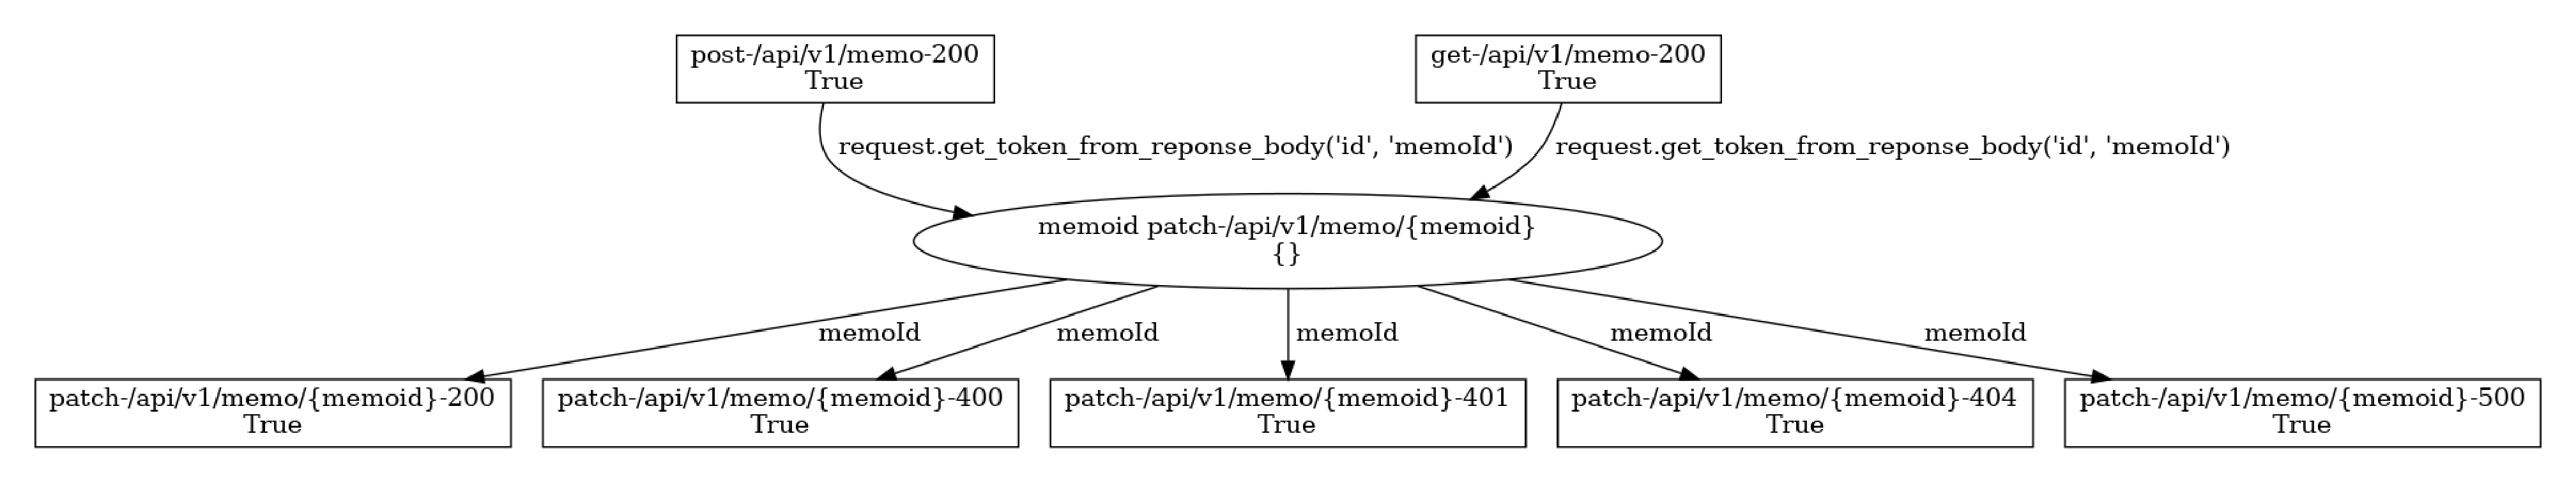
\includegraphics[width=\columnwidth]{figures/memos-0-initial-state.pdf}
    \caption{Initial state of the CPN, result of the {\tt Memos} OpenAPI transformation.}
    \label{fig:Memos_attack_case_a}
    \end{subfigure}

    \begin{subfigure}{\textwidth}
    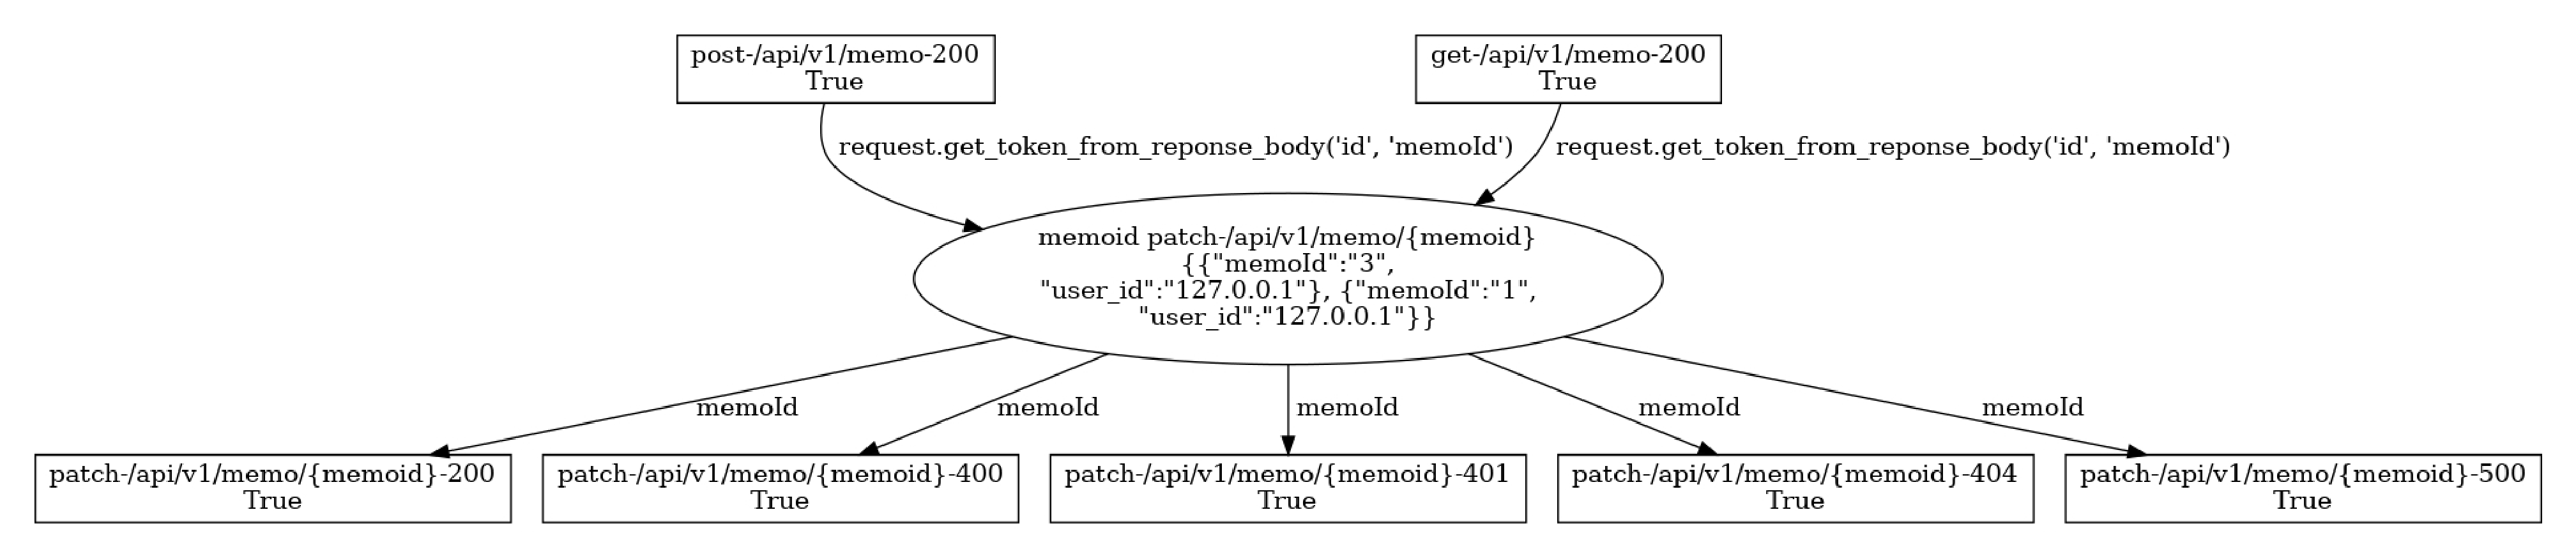
\includegraphics[width=\columnwidth]{figures/memos-line-9-fire-line.pdf}
    \caption{CPN state after processing line 11}
    \label{fig:Memos_attack_case_b}
    \end{subfigure}
\end{figure*}

\begin{lstlisting}[caption={Error message displayed when verifying with the CPN obtained after the transformation the log file containing the BOLA attack carried out.},captionpos=t,basicstyle=\ttfamily\small, label={lst:memos_error_msg},frame=single,breaklines=true]
Fire error, line 11:  transition not enabled for 
{
   "memoId->"{
      "memoId":"None",
      "user_id":"127.0.0.1"
   },
   "request->"{
      "uri":"/api/v1/memo/6",
      "method":"PATCH",
      "user_id": "127.0...."}
}
\end{lstlisting}


\subsection{Threats to Validity}

This section discusses the threats to validity that we have identified for this study~\cite{RH-ESE-09} according to construct, internal, external validity, and reliability.

\subsubsection*{Construct Validity}

We have conducted controlled experiments that allowed us to fine-tune our tool and measure the metrics of interest. In this sense, no problem should arise from our experiential study. 

\subsubsection*{Internal Validity}

Since we are not examining causal relationships in the results obtained, our study is free from threats to internal validity.

\subsubsection*{External Validity}

Our approach is tied to a concrete OpenAPI specification. Therefore, our approach may need to be adapted to future OpenAPI specifications. Also, we assume that the web server logs that are necessary for the replay algorithm are centralized. This extent, however, is discouraged in network administration, where the principle of network segmentation (as a way to reduce the number of assets in a network segment, limiting lateral movements of potential attackers) is commonly recommended~\cite{NetSegmentation-book-19}.

Similarly, {\nameTool} currently works with the JSON file generated after parsing the web server logs. Therefore, it would be necessary to adapt our tool to analyze the log files of other web servers.

As for our user-based assessment, it is true that there is no population from which a statistically representative sample has been drawn. However, as we use it as case studies, we can conclude that the results are extensible to cases that have common characteristics and therefore the findings are relevant.

\subsubsection*{Reliability}

Our tool, the running example, and the results of our user-based evaluation are publicly accessible through our GitHub repository~\cite{links2cpn}. Therefore, other researchers can perform the same study later and the results would be the same.

